\subsection{ÜB-Tipps}

\begin{frame}{Ordnungsrelationen}
	
	\only<1>{\begin{itemize}
		\item Eine Halbordnung auf der Menge $M$ ist eine reflexive, antisymmetrische, transitive, binäre Relation auf $M$
		\item Eine Totalordnung auf der Menge $M$ ist eine Halbordnung, welche zusätzlich total ist
	\end{itemize}}
	\only<2->{\begin{itemize}
		\item \textcolor{black!40}{Eine Halbordnung auf der Menge $M$ ist eine reflexive, antisymmetrische, transitive, binäre Relation auf $M$}
		\item \textcolor{black!40}{Eine Totalordnung auf der Menge $M$ ist eine Halbordnung, welche zusätzlich total ist}
	\end{itemize}}

	\visible<2->{\medskip
	Den Kram definieren wir später irgendwann korrekt, aber ist jetzt erstmal nicht wichtig...
	}

\end{frame}

\begin{frame}{Ordnungsrelationen}

	\begin{columns}
		\begin{column}{.6\textwidth}
			Anschaulicher: \begin{itemize}
			\item Bsp. Totalordnung: $\le$ auf $\nZ_n$ \begin{itemize}
				\item Man kann alle Elemente miteinander vergleichen
				\item Für zwei Elemente $x,y \in \nZ_n$ gilt $x \le y$ oder $y \le x$ 
				\item Elemente lassen sich als Kette durch $\le$ verbunden darstellen
				\item Hier genau ein Minimum (nämlich $0$) und ein Maximum (nämlich $n-1$)
			\end{itemize}
			\end{itemize}
		\end{column}
	
		\begin{column}{.4\textwidth}
			\centering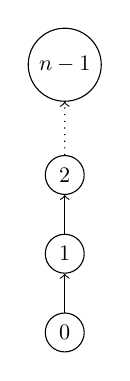
\begin{tikzpicture}[every node/.style={scale=.8,draw,circle}]

				\node (n-1) at (0,3.4) {$n-1$};

				% \node (dots) at (0,3) {\vdots};

				\node (2) at (0,2) {$2$};
				\node (1) at (0,1) {$1$};
				\node (0) at (0,0) {$0$};

				\draw[->] (0) -- (1);
				\draw[->] (1) -- (2);
				% \draw[->] (2) -- (dots);
				\draw[->,dotted] (2) -- (n-1);

			\end{tikzpicture}
		\end{column}
	\end{columns}

	

\end{frame}
	
\begin{frame}{Ordnungsrelationen}

	\begin{columns}
		\begin{column}{.6\textwidth}
			Anschaulicher: \begin{itemize} 
			\item Bsp. Halbordnung: $\subseteq$ auf $\Pot(M)$ mit bel. $M$ \begin{itemize}
				\item Es gibt Elemente $X,Y \in \Pot(M)$, für die weder $X \subseteq Y$ noch $Y \subseteq X$ gilt
				\item Elemente lassen sich als Hasse-Diagramm darstellen, aber i.A. nicht als Kette
				\item Hier genau ein Minimum (nämlich $\emptyset$) und ein Maximum (nämlich $M$)
			\end{itemize}
		\end{itemize}
		\end{column}
	
		\begin{column}{.4\textwidth}
			\centering\begin{tikzpicture}[every node/.style={scale=.8}]
				\tikzmath{\colsep=1.5;\rowsep=1;}

				\node (a-b-c) at (0,0) {$\set{a,b,c}$};

				\node (a-b) at (-\colsep,-\rowsep) {$\set{a,b}$};
				\node (a-c) at (0,-\rowsep) {$\set{a,c}$};
				\node (b-c) at (\colsep,-\rowsep) {$\set{b,c}$};

				\node (a) at (-\colsep,-2*\rowsep) {$\set{a}$};
				\node (b) at (0,-2*\rowsep) {$\set{b}$};
				\node (c) at (\colsep,-2*\rowsep) {$\set{c}$};

				\node (empty) at (0,-3*\rowsep) {$\emptyset$};

				\draw[->] (a-b) -- (a-b-c);
				\draw[->] (a-c) -- (a-b-c);
				\draw[->] (b-c) -- (a-b-c);
				\draw[->] (a) -- (a-b);
				\draw[->] (b) -- (a-b);
				\draw[->] (a) -- (a-c);
				\draw[->] (c) -- (a-c);
				\draw[->] (b) -- (b-c);
				\draw[->] (c) -- (b-c);
				\draw[->] (empty) -- (a);
				\draw[->] (empty) -- (b);
				\draw[->] (empty) -- (c);


			\end{tikzpicture}
		\end{column}
	\end{columns}	

\end{frame}

\begin{frame}{Notwendig und Hinreichend}
	\begin{block}{Def.: Notwendige Bedingung}
		Eine \textbf{notwendige Bedingung} zu einer Aussage $K$ ist eine Aussage $A$, für die gilt:

		{\center $K$ kann nur erfüllt sein, wenn die Bedingung $A$ gilt.}
		\\[0.5em]
		Das heißt \textit{nicht}, dass $K$ erfüllt sein muss.
	\end{block}

	\begin{block}{Def.: Hinreichende Bedingung}
		Eine \textbf{hinreichende Bedingung} zu einer Aussage $K$ ist eine Aussage $B$, für die gilt:
		\center Wenn die Bedingung $B$ erfüllt ist, so ist garantiert auch $K$ erfüllt.
	\end{block}
\end{frame}